\begin{figure*}[thb!]
  \caption{Approach overview}
  \centering
  \label{fig:approach}
  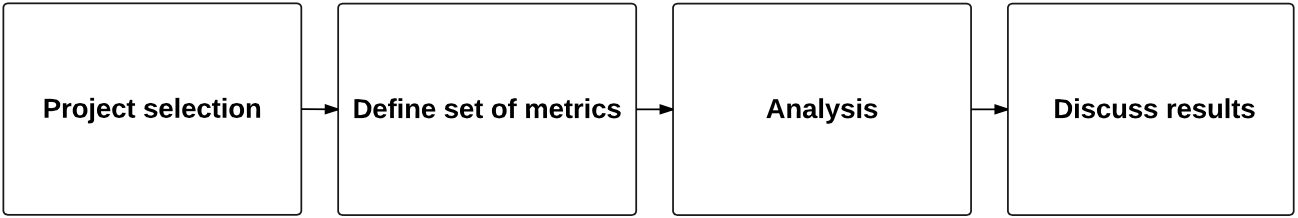
\includegraphics[width=1\textwidth]{figures/approach}
\end{figure*}

The goal of our project is to distinguish Defect Debt from Bugs. In order to do that we conducted a study using one large open source project, Google Chrome. We present our approach overview in \ref{fig:approach}. First, we extract data from the source code and from the issuer tracker repositories. Second,  we process the data to find relevant attributes and link them together. Third, we define our set of metrics and models. Then we analyze our results and answer the research questions. In the following sections we explain in details each one of the steps in our approach.   

\subsection{Data Extraction}

We use Google Chrome to conduct our study. Chrome is a large, mature open source software mostly written in C/C++. The criteria to select this project are its size, the easy access to its source code repository and to the its issuer tracker. Other than that, we had at our disposal some of the desired data that was used in a previous study. This data contained 47.938 html files and 5 tables. Each one of the files represent a bug extracted from the issue tracker. The tables contains the necessary information to link issues files, bugs and commits together. 

To complement the data necessary to our study, we extract from the Chrome Releases website \ref{chrome_releases} the release date of each stable version release, the tag of the release and the release number. Then we store this data in our database.
 
In order to have all the source code available we clone Chromium Git repository. 

\subsection{}


the issues files the the bug reported date and the number of comments that 